\chapter{Android Dynamic Native Code}\label{chapter:android_dynamic_native_code}

This chapter will cover shortly how to write native code in Android and how
the connection between Java and C/C++ is being established as well as its
integration into Android Studio.
Then there will be a sample application that shows a dynamic native code execution of a native code shared library, a binary or even machine code that can either be shipped within \code{assets/} or can be pulled in from external sources like the web, secure elements and so on. It will also be covered
if and to what extent an Android App has access to its own memory location as
well to its mapped files considering its writing and execution permissions.
With C/C++ there should be multifarious possibilities if sandboxing/permission concept mechanisms do play along.

\section{NDK and Android Studio Integration}\label{section:ndk_integration}
A complete documentation and starting guide about the NDK can be found at \parencite{ndk} and a guide to the integration into Android Studio at \parencite{ndk_integration}.
There is more than one way to integrate the NDK into Android Studio. The one described
in this thesis uses the platform build tools script \code{ndk-build}. Another possible
integration is the use of the Gradle experimental plugin and is described in \parencite{gradle_experimental}.
The NDK allows to embed compiled C/C++ in an application. It can be installed via Android Studio which is the default and recommended IDE for Android development.
The result of compiled C/C++ code is of course CPU dependent. Therefore the library has to be cross compiled for
every possible CPU supported by Android. Possible architectures supported by the NDK are so far:
\begin{itemize}
\item \textbf{arm64-v8a}
\item \textbf{armeabi}
\item \textbf{armeabi-v7a}
\item \textbf{mips}
\item \textbf{mips64}
\item \textbf{x86}
\item \textbf{x86\_64}
\end{itemize}
The common way is that Android compiles every native source code into shared libraries
(\code{*.so}) that can then be loaded from Java code. However, it is also possible to build executable binaries with NDK in theory. Entry point for the build process is an \code{ndk-build} script inside of the installed \code{ndk-bundle/} folder that takes care of calling the cross-compiling toolchains. It can be controlled by Android makefiles (\code{Android.mk}) and does
expect a specific folder structure to work which is partially created when using Android Studio. An additional \code{jni/} folder has to be created that will hold all the native source code (right click on \code{app/} and choose \code{New->Folder->JNI Folder}).

From Java, the compiled library can be loaded by using a
\code{System.loadLibrary("MyLib")} call. In order to be able to call methods out
of that library, the method signatures have to be known and can be declared with
a \code{native} keyword in addition to the common Java method declaration. It is also a
common practice to create a new Java class specifying all NDK functions but not a must have. When doing so, a header file for the native source code (\code{*.h}) can be automatically
created by using the \code{javah} command line tool. It includes the necessary JNI
declarations for the specified methods (including the JNIEnv pointer for instance)
and can then be included in the C/C++ source file that can then be implemented as a
usual C/C++ project.

The last necessary thing is to create an \code{Android.mk} makefile for every library as well as \code{Application.mk}. The \code{Android.mk} file defines the library name that \code{loadLibrary()} expects, lists the source files and defines the outcome (shared library or executable) whereas \code{Application.mk} includes
the libraries to build (\code{APP\_MODULES}) and the architectures to build for
(\code{APP\_ABI}). The \code{build.gradle} has to be adapted as well, defining the
outcome directory path relative to \code{jni/} and \code{android.useDeprecatedNdk = true} needs to be added to \code{gradle.properties} to suppress an error message.
A \code{ndk-build} call will then compile all sources and creates the libraries
at \code{libs/<archs>}. They can be used out of the box without need to load them by hand
at runtime. All that's needed is the \code{loadLibrary()} call. Physically, those libraries are stored at the same path as the App APK file like introduced earlier. By applying this method, those native libs are shipped together within the application that might not be the intended behavior. A whole NDK sample project with those necessary
pointed out adaptations is shown in \autoref{chapter:ndk_sample_project}.

\section{Dynamic Shared Library Loading out of a File}\label{section:shared_library_loading}
The process demonstrated in \autoref{section:ndk_integration} is common practice to
integrate native code into an App but is not really dynamically loaded. Instead
the main idea of dynamical code loading is the distribution of code for instance
after licensing the App or to apply some sort of copy protection mechanisms by hiding
the true functionality. One approach is to use native code as a loading mechanism.
C/C++ has the ability to load shared objects (\code{*.so}) with a method called
\code{dlopen()} (=``Dynamic Library Open''). Its signature is shown in \autoref{dlopen_sig}.
\begin{lstlisting}[language=C++, caption=dlopen() Signature, label=dlopen_sig]
void *dlopen(const char *path, int flag)
\end{lstlisting}
Obviously, a path to the library file is needed as well as a flag that defines the binding of variables and methods (lazy, global, \ldots see \code{dlopen()}-reference for more information).
But what path should and can be used in the context of Apps? A path inside of the APK
for instance is not reference-able as a path string. So generally Apps can use different storage options that are listed and shortly described and can also be looked up in
\parencite{storage_options}.
\begin{itemize}
\item \textbf{Shared Preferences} can store data in form of key-value pairs
\item \textbf{Internal Storage} stores private arbitrary data on the device memory at the path
 \code{/data/data/<appPackage>/} that is only accessible by the App itself.
\item \textbf{External Storage} can also store arbitrary data on \code{/sdcard/} but it is not exclusively readable by the initializing App and needs a permission declaration in
the manifest file.
\item \textbf{SQLite Database} provides support for powerful private databases
\item \textbf{Network Connection} can store data on the web
\end{itemize}
The most suitable option should be the internal storage since the App has unlimited read/write rights and the content is safe from other sources rather then itself. For simplicity and demonstration reasons, the library to load will be stored in the
\code{assets/} folder of the App that also only exists in the APK but is not
reference-able through a path but can be opened through an Asset-Manager. It will therefore be copied into the internal storage first. \autoref{internal_init} shows the Java initialization of the path to the final library to load. The \code{getDir()} call generates a new folder within the internal App storage and a file container for the library to load gets created.
\begin{lstlisting}[language=Java, caption=Internal Storage Initialization, label=internal_init]
File internalStoragePath = new File(getDir("dynamic", Context.MODE_PRIVATE), "mul.so");
\end{lstlisting}
At a next step, the library has to be copied out of the assets folder and into that
recently created file container for it. Any file within the assets can be opened with an
\code{getAssets().open("file")} call. For the read/write process one can use
\code{BufferedInputStream} and \code{BufferedOutputStream}, shown in
\autoref{buff_in_out}.
\begin{lstlisting}[language=Java, caption=Buffered Input/Output, label=buff_in_out]
BufferedInputStream bis = null;
OutputStream soWriter = null;
final int BUF_SIZE = 8 * 1024;
try {
    bis = new BufferedInputStream(getAssets().open("mul.so"));
    sWrite = new BufferedOutputStream(new FileOutputStream(internalStoragePath));
    byte [] buf = new byte[BUF_SIZE];
    int len;
    while ((len = bis.read(buf, 0, BUF_SIZE)) > 0){
        sWrite.write(buf, 0, len);
    }
    sWrite.close();
    bis.close();
} catch (IOException e) {
    e.printStackTrace();
}
\end{lstlisting}
Now the program is ready to transform the transition into the native (C/C++) world.
The signature of the native method to call does contain at least the path as a string to
the internal stored file that can be printed with a \code{getAbsolutePath()} call of the
\code{internalStoragePath} file object. Remember that \code{dlopen()} needs that path.
A class ``\code{MyNDK}'' gets created and contains the native declaration of the
``\code{libExe(String path)}'' method as well as a static call of
\code{System.loadLibrary(``MyLib'')} that takes care of the binding.
The implementation of \code{libExe()} is shown in \autoref{libexe}.
\begin{lstlisting}[language=C++, caption=Native libExe(), label=libexe, numbers=left]
JNIEXPORT void JNICALL Java_ma_schleemilch_nativestuff_MyNDK_libExe
        (JNIEnv * env, jobject jobj, jstring path){
        const char *libpath = env->GetStringUTFChars(path, NULL);
        LOGD("Received Path: %s", libpath);
        void* handle;
        const char* error;
        long (*mul)(int, int);

        handle = dlopen(libpath, RTLD_LAZY);
        if (!handle) {
                LOGE("DL Open failed: %s", dlerror());
                return;
        }
        dlerror();
        *(void**)(&mul) = dlsym(handle, "mul");
        if ((error = dlerror())!= NULL) {
                LOGE("DL Error after DLSYM: %s", error);
                return;
        }
        LOGD("# 9*5 = %ld", (*mul)(9,5));
        dlclose(handle);
        remove(libpath);
}
\end{lstlisting}
One short word about logging/debugging: The common \code{printf()} writes to the standard output. A better way of viewing C++ outputs is to use the ADB logging mechanism. Google does include a \code{\_\_android\_log\_print()} function that
has the same behavior as \code{printf()} but writes to the Logcat output and
\code{LOGD()} is a defined makro calling that function.

The library that will get loaded is a simple multiplication function and a pointer
for it gets initialized at line seven. \code{dlopen()} returns a void pointer and
\code{dlsym()} searches the symbol table of the handle pointed file for the function
given as a string. That call is interesting when comparing C to C++. In
\parencite{dlopen_howto}, the problem of name mangling in C++ and the combined usage of
\code{dlopen()} is being described in detail.
In short, one will need an ``\code{extern "C"}'' at the \code{mul()} definition in order to make the \code{dlsym()} function to find the method
because C++ does not use only the method name as its symbol but a unique created ID.
So without that extern keyword, \code{dlsym()} will fail.
Finally, the \code{mul()} function can be called out of the library.
After that call, \code{dlclose()} has to be executed. It is also possible to remove
the library file after that process that might be useful for copy protection usage.
From the Java perspective, a \code{MyNDK} object needs to be created followed by
a call of its \code{libExe()} to call and execute the library.

To be able to load a shared object library like this, it obviously needs to be
generated first. One could use an own cross compiler for that or just also use
the NDK since it includes all necessary tool-chains.
However, some project structure changes have to be made to be able to compile two independent libraries. Each library to compile should have its own folder inside
of \code{jni/} with an \code{Android.mk} each. The greater \code{Android.mk} in
\code{jni/} has to be changed to call all subsequent make files with
``\code{include \$(call all-subdir-makefiles)}'' and each module to build has to be
added to \code{Application.mk} as well. Gradle needs to know the names of the sub
directories of \code{jni/} so that ``\code{jni.srcDirs=[]}'' has to be
filled with those folder name strings. As a result of that structure, the compiled
library that will get loaded afterwards also will be saved in the \code{libs/} folder
and shipped within the App when not deleting it. In a scenario where an App requests new
parts and gets them from a server for instance, these libraries should then only be
present server sided. In order to receive the right compiled shared object for every
device, it should add CPU information with its request (e.g. by sending the output
of ``\code{System.getProperty("os.arch")}'').

It is also possible to do that kind of shared object loading directly out of Java
code. Like shown in \autoref{section:ndk_integration}, a static call of
\code{System.loadLibrary("MyLib")} does the heavy lifting of invoking the library.
The \code{loadLibrary()} function however does only check specific paths for the given
library name which are specified in \code{java.library.path}, containing
\code{/vendor/lib} and \code{/system/lib} as well as the path of the App's APK lib
folder. So for dynamic loading, this loading method is not suitable since these
locations can't be accessed unless with root rights. Fortunately there is another
loading function \code{System.load(String s)} that accepts an absolute path to
the shared object file like the C++ equivalent \code{dlopen()}. Attention must be
paid to naming conventions in \code{loadLibrary()} in comparison to \code{load()}.
Libraries compiled by the NDK are getting a \code{lib} prefix to its actual module
name automatically. It means that \code{System.loadLibrary("MyLib")} invokes a file
that's called \code{libMyLib.so} while the \code{load()} needs directly the physical
stored path name.

Even if Java is also capable of loading shared object libraries at runtime, the
signatures of the library to load has to be implemented before to be able to call
its methods unlike the C/C++ implementation where symbols can be resolved itself.

It can also be tried to call a whole native activity with the C/C++ method since
a native activity project can be also compiled into an shared object (see NDK
examples ``native-activity''). To invoke the activity, one need to call the
\code{android\_main()} method but when doing so, it turns out that it will cause
a segmentation fault (SIGSEV).


\section{Dynamic Binary Execution out of a File}\label{section:dyn_bin_exec}

It could be also interesting to execute binaries directly instead of loading shared objects. To compile them, again the NDK can be used with changing the module's
\code{Android.mk} file by replacing \code{include \$(BUILD\_SHARED\_LIBRARY)} with
\code{include \$(BUILD\_EXECUTABLE)}. When doing so, there is to mention
that all modules compiled for 32 Bit systems are executables directly while modules
compiled for 64 Bit are again shared objects (by checking the output of the Linux
\code{file} command line program).
They are dedicated to their interpreters (\code{/system/bin/linker} and \code{/system/bin/linker64}) that will execute them. It does however make a difference since
Android seems like to support only position independent executables (PIE).
PIE's purpose is to be able to execute its code regardless of its absolute address
and \parencite{pie} is an interesting article about the impact of PIEs.
Shared objects are a specific implementation of PIEs. So in case of 32 Bit systems, there will be an error message
``\code{error: only position independent executables (PIE) are supported.}'' when
compiled as executable without any additions. There is of course a solution for that
by adding a \code{LOCAL\_CFLAGS} entry \code{-fPIE} as well as the \code{LOCAL\_LDFLAGS}
entries \code{-fPIE} and \code{-pie} to its Android makefile. In fact, after adding
those attributes, there is no more difference between that compiled executable
compared to the shared library counterpart other than it has to contain a
\code{main()} in order to be executed.

Again, binary execution can be implemented in Java as well as in native C/C++ code.
Java will be used in both cases to fetch the binary file from an arbitrary location that can be determined at runtime or statically (again \code{assets/}
for demonstration) and writing it into the internal private storage path. By checking the outcome file of that process via \code{adb shell} and ``\code{ls -l}'', the file is of course not marked as executable by default but at least the owner and the group is set right so there
should not be any permission issue.
If the file is not marked as an executable, it will result in a ``can't execute: Permission denied'' message in case of a C++ implementation or an ``IOException'' in case of Java. Fortunately, it can be fixed simply by calling \code{setExecutable(true)}
of the Java \code{File} object representing the binary.

\subsection{Java Implementation}\label{dyn_bin_java}
The preparation procedure for executing is the same like in the shared object loading
case, means saving the file in its internal storage and delivering a \code{File} object
to work with. A Java \code{Runtime} object has an \code{exec(String s)} function that is capable of execution code given at its absolute path. It does return a \code{Process}
object. At Android, the current runtime can be accessed with a static access of the
\code{Runtime}'s \code{getRuntime()} function.
That's basically everything needed to make it work. However one will not see any
outputs (like \code{printf()}) of that separately started process.
The documentation of \code{Process} reveals that the subprocess output can be
fetched with \code{getInputStream()} and its error output with \code{getErrorStream()}.
It can also be checked and waited for the subprocess to finish via \code{waitFor()}
which should be the normal case when calling a native binary. The final very
compact implementation is shown in \autoref{java_bin_exec}.
\begin{lstlisting}[language=Java, caption=Java Native Exec(), label=java_bin_exec]
Process nativeExe = Runtime.getRuntime().exec(internalPath);
BufferedReader reader = new BufferedReader(new InputStreamReader(nativeExe.getInputStream()));
int read;
char[] buffer = new char[4096];
StringBuffer output = new StringBuffer();
while ((read = reader.read(buffer)) > 0) {
    output.append(buffer, 0, read);
}
reader.close();
// Waits for the command to finish.
nativeExe.waitFor();
String nativeOutput =  output.toString();
Log.d(TAG, "nativeOut: " + nativeOutput);
\end{lstlisting}

\subsection{C/C++ Implementation}\label{dyn_bin_c}
As for C/C++, the implementation is not much more complicated compared to Java.
The main part of execution is a call of \code{popen()}
(man printed at \parencite{popen}) which expects a command
given as a char array to execute and the type of its created pipe (read ``r'' or write ``w''). Internally, it uses \code{fork()} and \code{pipe()} for creating the new
process and executing the given program at its path. It returns a \code{FILE} pointer
whose stream can be read out by \code{fgets()}. The complete C++ implementation
of the behavior is shown in \autoref{cpp_bin_exec}. In order to catch \code{stderr}
the program path string can be extended with the string ``2>\&1'' to detour the error
channel (2) to the common output channel, \code{stdout} (1).
\begin{lstlisting}[language=C++, caption=C++ Native Exec(), label=cpp_bin_exec]
JNIEXPORT void JNICALL Java_ma_schleemilch_nativestuff_MyNDK_binExe (JNIEnv *env, object obj, jstring path)
{
	const char *exepath = env->GetStringUTFChars(path, NULL);
	FILE* fpipe;
	char* command = new char[strlen(exepath) + strlen(" 2>&1") + 1];
	int ind = 0;
	for (int i = 0; i < strlen(exepath); i++){
		command[ind] = exepath[i];
		ind++;
	}
	command[ind++] = ' ';
	command[ind++] = '2';
	command[ind++] = '>';
	command[ind++] = '&';
	command[ind++] = '1';
	command[ind++] = '\0';
	char line[256];
	if (!(fpipe = (FILE*)popen(command, "r"))) return;
	while(fgets(line, sizeof(line), fpipe)){
		LOGD("%s", line);
	}
}
\end{lstlisting}

\section{Dynamic Code Execution out of Memory}\label{section:dyn_code_memory}

Until now, dynamic code execution or loading via shared libraries was done
by downloading/copying a file into the internal storage of the App followed
by invocation. This seems like a detour since at some point, that file has to be fetched and written to a file followed by loading it again.
Instead, it would be also interesting if program code can be executed directly
out of memory. Memory in this context means the RAM region of the App's process.
So there needs to be inspected if an Android App process has even access
to memory and if it is feasible to read/write/execute program code in self
allocated memory.

\subsection{Android Memory Mapping}\label{section:memory_mapping}
So let's have a look at the general memory mapping of a common Android App.
When printing the content of \code{/proc/<PID>/maps} of the App's Linux process, virtual memory locations that are assigned to the process are revealed.
The keyword ``\code{self}'' is the specific PID that can be used as a path in a process to access its own \code{proc/} directory (Otherwise, root rights are
needed to read maps of processes other than its own).
An example output of one map entry is shown in \autoref{tab:proc_maps_out} and its explanations are pulled out of a stack-overflow answer to the question at \parencite{proc_maps}, that explains the contents of the maps output.
\begin{table}[htb]
  \caption[Content of /proc/<PID>/maps]{Content of /proc/<PID>/maps}
  \label{tab:proc_maps_out}
  %\centering
  \texttt{
  \begin{tabular}{l l l l l l}
    \toprule
    address & perms & offset & dev & inode & pathname \\
    \midrule
    6feed000-708ca000 & rw-p & 00000000 & b3:1c & 105876 & /data/.../framework@boot.art \\
    \bottomrule
  \end{tabular}
  }
\end{table}
The \code{address} shows the absolute physical start and end of its mapped section. Permissions (\code{perms}) informs about how this region can be accessed (common Linux ``\code{rwx}'' permission triple)
and can be marked as private \code{p} (exclusively accessible by its mapped process) or shared \code{s} (accessible from other processes).
If the section was mapped out of a file, \code{offset} describes the offset
in bytes to the specific region of the mapped file.
Device (\code{dev}) also only applies if mapped from a file and includes
the device number while \code{inode} holds its file number.
The \code{pathname} obviously shows the path of its source file.

When looking at an Android App process in particular, it reveals all kind of mapped libraries (which is a great amount even with a blank activity App and emphasizes that forking of Zygote is way more efficient), fonts, its own \code{base.apk} as well as  regions that don't have a pathname or just a pseudo pathname like ``\code{[anon:linker\_alloc]}'' or ``\code{[stack]}''.

Generally, a stack contains data that only persists inside of a function call like initialized arrays or variables and its content gets automatically released after returning from that function.
The heap however can be used by the programmer to allocate memory
(e.g. with \code{malloc()}) manually but has to be freed explicitly.
Let's evaluate which mapping sections are used to store heap as well as common stack elements by creating a native function with a buffer using \code{malloc()} and also a common local integer variable.
While \code{malloc()} creates memory areas
without any additional adaption, \code{mmap()} can map a whole file, returns a pointer to its start address and can set memory protection flags of the mapped area that are necessary when it shall be executed, written or read later
(\code{PROT\_EXEC}, \code{PROT\_READ}, \code{PROT\_WRITE}).
Executing code out of heap is forbidden by default.
\autoref{r_maps} shows how to read and print the maps content from C++ on Logcat.
\begin{lstlisting}[language=C++, caption=Reading /proc/self/maps, label=r_maps]
FILE* fp;
char line[2048];
fp = fopen("/proc/self/maps", "r");
if (fp == NULL){
    LOGE("Could not open /proc/self/maps");
    return;
}
LOGD("Before:\n");
while (fgets(line, 2048, fp) != NULL) {
    if (strstr(line,"triggeredString")){
        LOGD("%s", line);
    }
}
fp->_close;
\end{lstlisting}
Unfortunately, the amount of output lines is limited when using logging via Logcat which
implements a ring buffer with a device dependent size (``\code{adb logcat -g}''). That
is a problem when printing the whole memory mapping and can confuse the inspection
since a ring buffer overwrites itself when overflowing. So either one can use an adb shell to ``\code{cat /proc/<PID>/maps}'' by hand (root rights needed)
or triggering the Logcat output to specific strings. Getting an overview via a whole output and triggering for specific parts via Logcat afterward might be the best solution.
To find the mapping of the executing library, triggering the name library is enough
and its output is shown on top of \autoref{tab:mem_alloc_map}. Three regions
of the library are mapped, for reading, writing and executing each.
\begin{table}[htb]
  \caption[Memory Allocation Mapping]{Memory Allocation Mapping}
  \label{tab:mem_alloc_map}
  %\centering
  \texttt{
  \begin{tabular}{l l l l l l}
    \toprule
    address & perms & offset & dev & inode & pathname \\
    \midrule
    b39f5000-b39f8000 & r-xp & 00000000 & b3:1c & 187593 & .../app/.../lib/arm/libMemory.so \\
    b39f8000-b39f9000 & r--p & 00000000 & b3:1c & 187593 & .../app/.../lib/arm/libMemory.so \\
    b39f9000-b39fa000 & rw-p & 00000000 & b3:1c & 187593 & .../app/.../lib/arm/libMemory.so \\
    be0c3000-be8c2000 & rw-p & 00000000 & 00:00 & 0      &    [stack]\\
    b3940000-b39c0000 & rw-p & 00000000 & 00:00 & 0      &    [anon:libc\_malloc]\\
    \bottomrule
  \end{tabular}
  }
\end{table}
When creating an integer variable and printing its address afterwards, it appears
that it is located in a ``\code{[stack]}'' marked region that is not included in
the library mapped range and memory allocations by the \code{malloc()} as well as the
\code{mmap()} function are listed in areas marked as ``\code{[anon:libc\_malloc]}''
(also printed in \autoref{tab:mem_alloc_map}).

\subsection{Code Execution}\label{section:code_execution}
So which function (malloc or mmap) is more suitable for just in time (JIT) code execution?
Like explained in \parencite{jit_intro}, one should go with \code{mmap()} over \code{malloc()}. This is about protection bits that can only be set at memory page boundaries.
That's why with \code{malloc()}, it needs to be ensured manually that the allocation is aligned at a page boundary. If it is not the case, a \code{mprotect()} call will have the side effect of disabling/enabling more memory than actually required.
Since \code{mmap()} is designed for mapping whole files, it will take care of that by default.

In the end, ``code'' like in ``Executing Code'' stands for machine code that will get executed, which is not more than a sequence of bytes (actually only 1's and 0's).
Until this point, dynamic loading was performed through files that do have a specific format that contains far more than just raw bytes that are getting
executed (like shared objects or ELF binaries, partially described in
\autoref{section:elf_file_format}) and API calls.
There is of course a reason for those kind of formats since they do offer information for the linker to function properly on every system using them.
Generally there are two possibilities of invoking and executing
code and in the end native instructions.
The first one is to map a well known format like a shared object or an executable
into memory but then the running ``host'' process needs to be adapted in order to find those executable parts in memory (linker is responsible for doing that before the program gets executed).
If a program is using external libraries, a linker is responsible for linking them in, statically or dynamically. So one would end up writing linker
functionalities or patching the one mapped into the process. It does exist a proof of concept for a Linux x86\_64 system shown in \parencite{memdlopen} that can load
shared objects out of a file or an Internet socket right into the process space.
A key part of this program is the patching of ``\code{ld-2.19.so}'' that is already mapped within the process. Porting that library to Android is not that simple since Android is not using this library but an own linker at \code{/system/bin/linker}.

So let's first try to invoke machine code directly without any file format overhead like
in ELF binaries and shared objects. Again, a simple multiplication function will be implemented to show a proof of concept, shown in \autoref{machineCodeMulC}.
\begin{lstlisting}[language=C, caption=machineCodeMul.c, label=machineCodeMulC]
int mul(int a, int b){
    return a*b;
}
\end{lstlisting}
This time, a cross-compiler and its included tools like \code{objdump} is useful.
For this explicit purpose, the \code{arm-none-eabi} tool-chain was being used in
combination with an Arch Linux 64 Bit system.
It does contain a \code{gcc} to compile C-Code as well as \code{objdump} to analyze object files.
A ``\code{arm-none-eabi-gcc -O3 -c machineCodeMul.c -o machineCodeMul.o}'' call outputs an object file out of a C source.
Objdump can then show mnemonics as well as its corresponding machine code
for every function, exactly what will then be written to memory in the next step
(output for \code{machineCodeMul.o}'s \code{mul()} function shown in \autoref{tab:mul_objdump}).
\begin{table}[htb]
  \caption[arm-none-eabi-objdump -D machineCodeMul.o]{arm-none-eabi-objdump -D machineCodeMul.o}
  \label{tab:mul_objdump}
  %\centering
  \texttt{
  \begin{tabular}{l l l l}
  \toprule
  \multicolumn{4}{l}{00000000 <mul>:}\\
  \midrule
  0: & e0000091 & mul & r0, r1, r0 \\
  4: & e12fff1e & bx  & lr \\
  \bottomrule
  \end{tabular}
  }
\end{table}
The byte sequence \code{0xe0000091} represents the raw machine code for the mnemonic equivalent of a multiplication
(\code{r0 = r1 * r0}) and the following one is responsible for exiting the function and returning the value. Since object files are normally little endian, the bytes written
to memory have to be reordered first (\code{0xe0000091 turns to 0x910000e0}) before
execution.

At first, a memory location will be needed and therefore gets allocated,
a function for that purpose could be written that takes the regions size as an input like shown in \autoref{alloc_exe_mem}.
\begin{lstlisting}[language=C++, caption=alloc\_executable\_memory(), label=alloc_exe_mem]
void* alloc_executable_memory(size_t size) {
    void* ptr = mmap(0, size, PROT_READ | PROT_WRITE | PROT_EXEC, MAP_PRIVATE | MAP_ANONYMOUS, -1, 0);
    if (ptr == (void*)-1) {
        LOGE("mmap");
        return NULL;
    }
    return ptr;
}
\end{lstlisting}
It returns a void pointer to the starting address of its allocated region. Note that
if no file is being specified as a \code{mmap()} parameter (instead a ``\code{-1}''),
the \code{MAP\_ANONYMOUS} flag has to be set. Additionally, even though size can be specified in \code{mmap()}, its limited to page size constraints. So it will allocate
memory that is greater or equal to the given size. Note that there might be a
small security hole since that allocated memory is already marked as writable
and also that region is likely to be bigger than the actual code that will get
executed later. That could be exploited by an attacker. Therefore it is slightly more secure to allocate memory without execution  permission first since copying machine code to that location does only need write
permissions. The execution permission can be granted right before the function call
via \code{mprotect()}.

The next thing to do is to copy the bytes to be executed at that location. For that,
also a function seems suitable that takes a pointer, specifying some bytes and finally calling \code{memcpy()} (see \autoref{emit_code_mem}).
\begin{lstlisting}[language=C++, caption=emit\_code\_into\_memory(), label=emit_code_mem]
void emit_code_into_memory(unsigned char* m) {
    unsigned char code[] = {
        0x91, 0x00, 0x00, 0xe0, // mul r0,r1,r0
        0x1e, 0xff, 0x2f, 0xe1, // bx lr
    };
    memcpy(m, code, sizeof(code));
}
\end{lstlisting}
But how can this code actually be executed?
A \code{typedef} is being used to specify the function signature matching the C source function that will get executed afterwards.
It can get initialized by pointing to the allocated memory region like it also does when
writing a function the common way. The function name is then a pointer to the process region including the actual machine code.
After that, all that's left to do is calling it like a common function.
\autoref{exec_mach_code} shows the actual implementation via JNI C++ using the predefined methods from before and showing some additional output information about
the allocated memory spots.
\begin{lstlisting}[language=C++, caption=executeMachineCode(), label=exec_mach_code]
JNIEXPORT void JNICALL Java_schleemilch_ma_nativememory_MyNDK_executeMachineCode (JNIEnv *env, jobject obj){
    typedef int (*JittedFunc)(int, int);
    size_t SIZE = 8;

    void* m = alloc_executable_memory(SIZE);
    LOGD("MALLOC ADDR: %p", m);
    emit_code_into_memory((unsigned char*)m);

    JittedFunc func = (JittedFunc) m;
    LOGD("FUNC ADDR: %p", &func);

    int a = 20;
    int b = 4;
    LOGD("Result of %d * %d = %d", a, b, func(a, b));
}
\end{lstlisting}
Note that the function typedef variable \code{func} is just treated as a variable,
means its address relies on the stack region (like it is supposed to be)
and the \code{m}'s address allocated by \code{mmap()} is being displayed in the \code{/proc/self/maps} output without any ``\code{[libc\_malloc]}'' annotation or path but just left blank.

If the original C function does not contain any external library calls, the execution
of machine code directly out of memory is pretty straight forward, at least for one
specific function like showed for a multiplication. When library calls are being
performed inside of that method, it gets much more complicated. Even with function calls
within the same C file it is not a simple matter since linker functionality is
completely missing in this form of pure machine code. Therefore, addresses to jump to
have to be adapted by hand.

So in general, executing code out of memory is possible in Android ART but to be able
to use it productively, some more work has to be done in order to invoke whole shared
objects or whole binaries instead of machine code chunks like shown here. Just implementing an ELF parser at runtime to extract all kind of defined methods would not be enough but additional alterations to the machine code needs to be done to adjust jump addresses to the specific manually allocated memory containing machine code.

\section{Performance Comparison}\label{section:dyn_code_performance}
\autoref{tab:dyn_code_performance} shows a performance comparison
of described methods concerning dynamic code loading via DEX,
shared objects and executables using Java and C/C++. While
DEX and the shared object do rely on the same testing multiplication
function, the tested executable implemented a \code{printf()}.
That means that the measured values do not say anything about
invoking executables versus shared objects and DEX files but
something about the different implementation.
\begin{table}[htb]
  \caption[Dynamic Code Performance Comparison]{Dynamic Code Performance Comparison}
  \label{tab:dyn_code_performance}
  %\centering
  \texttt{
  \begin{tabular}{l c c c}
  \toprule
  Object to Load & Function & Loading Implementation & Time (ms)\\
  \midrule
  DEX & mul(int, int) & Java & 6-9 \\
  Shared object & mul(int, int) & Java & 3-4 \\
  Shared object & mul(int, int) & C/C++ & 2-4 \\
  \midrule
  Executable & printf() & Java & 23-27 \\
  Executable & printf() & C/C++ & 24-26 \\
  \bottomrule
  \end{tabular}
  }
\end{table}
Like expected, loading a method out of a DEX at runtime is significantly
slower (takes nearly twice as long) than invoking from a shared object.
The reason is the compiling step that has to be performed in order to produce the native code ODEX since ART can not execute DEX byte instructions.
However, the language used for invocation does not matter at all. That
also makes sense since Apps are being compiled by the ART VM at installation
time and the output is native code in both cases (Java or C++). Differences
should therefore only rely on the implementation of the transformation step -
means the compiler.

\section{General Memory Access}\label{section:general_mem_access}
In general, an App can write every memory section that is mapped with writing permission like expected. To find writable locations in the mapped space, again the output of \code{/proc/self/maps} can be used with triggering for the permission triple ``\code{rw-p}'' string. \autoref{gen_mem_write} for instance triggers for the specific writable \code{/system/bin/linker} entry. The size of the memory region can be parsed out of that matching line. ``\code{strtoll}'' can be used to do the actual parsing from a
hexadecimal char sequence to its ``\code{long long int}'' number and can be casted to a pointer (=memory address) afterwards.
Using a char pointer for the actual writing reading process
are commonly used, since char always has the size of one byte. So when using array notation, each byte of the memory can be easily accessed.
\begin{lstlisting}[language=C++, caption=memoryWriting(), label=gen_mem_write]
JNIEXPORT void JNICALL Java_schleemilch_ma_nativememory_MyNDK_memoryWriting
 (JNIEnv *env, jobject obj){
    FILE * fp;
    char line[2048];
    fp = fopen("/proc/self/maps", "r");
    if (fp == NULL){
        LOGE("Could not open /proc/self/maps");
        return;
    }
    while (fgets(line, 2048, fp) != NULL) {
        if(strstr(line, "rw-p 0001d000 b3:19 366") != NULL){
            LOGD("%s", line);
            break;
        }
    }
    fp->_close;

    char address[9];
    strncpy(address,line,8);
    address[8] = '\0';

    long long int mp = (long long int)strtoll(address, NULL, 16);
    void* vp = (void*)mp;
    char* cp = (char*) vp;
    LOGD("%p", cp);

    LOGD("Print/Write Memory:");
    for (int i = 0; i < 10; i++){
        LOGD("%x", cp[i]);
        cp[i] = i; //writing
    }
    LOGD("Print Memory:");
    for (int i = 0; i < 10; i++){
        LOGD("%x", cp[i]);
    }

}
\end{lstlisting}
Being able to write to memory in general is a necessary precondition for advanced patching techniques like adapting the linker and is therefore doable in ART.

\section{Utilizations}
The question is how those gathered methods of dynamically loading code can be
used practically. A few examples of how those dynamic code methods can be used
are shown here that are meant to inspire the reader for even more thought-through
advanced solutions.

\subsection{Licensing Improving}
Licensing is a common way of controlling additional paid
features of an App. The main problem of licensing mechanisms is the one
function call that checks the licensing status of its user. Like pointed
out in \parencite{app_sec}, the checking licensing call can be easily
patched, in many cases even automatically using Lucky Patcher or similar
software so that the function call always returns ``\code{licensed == true}''
or gets skipped entirely. How to solve this problem? A good practice would be to deliver necessary parts of an App only when the licensing mechanism was
called successfully, means that there was established a connection to the
licensing server for instance that in turn will distribute the additional
App content (see \autoref{fig:license_dynamic_loading}).
\begin{figure}[htb]
  \centering
  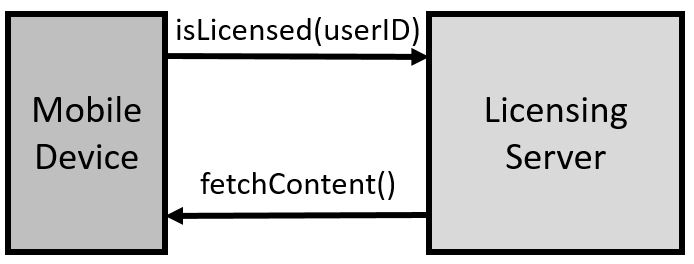
\includegraphics[scale=0.5]{figures/license_dynamic_loading}
  \caption[Dynamic App Content Loading]{Dynamic App Content Loading}
  \label{fig:license_dynamic_loading}
\end{figure}
So that even an attacker manages to skip the license call and fake the App
into being licensed, he still would not have access to those additional
functionalities cause of missing application files that will not getting
transmitted server sided. Like shown in this chapter,
that behavior could be implemented in native code as well as in Java and
is also relatively independent in terms of type of code to be loaded (DEX,
shared library, binary). However, if those additional App parts are being
downloaded successfully, with root rights they can be pulled out of the
device so that an advanced attacker could again circumvent the licensing
mechanism for several devices after purchasing the App once and then patching
the license/code fetching calls.
A possible remedy for that could be continuous license checking calls in the
background implemented as a service whenever there is an Internet connection
present (like every 10 minutes). That service could not only try to delete
files that should not be present at its device but could also lead to an
App crash with a meaningless message in case of not being licensed.

A simple way of crashing an application is to trigger a SIGSEV for instance
by accessing the NULL-pointer. In C/C++ that is no challenge since pointers
do exist (see \autoref{crash_app_sigsev}).
\begin{lstlisting}[language=C++, caption=crashApp(), label=crash_app_sigsev]
unsigned char *p = 0x00000000;
*p = 1;
\end{lstlisting}
That will cause an Android GUI message ``<AppName> has stopped working'' while
the ADB interface will reveal the actual cause ``Fatal signal 11 (SIGSEGV), code 1, fault addr 0x0 in tid 25271 (ma.nativememory)''.
 \begin{table}[htb]
   \caption[ADB SIGSEV Debugging]{ADB SIGSEV Debugging}
   \label{tab:sigsev_debug}
   %\centering
   \texttt{
   \begin{tabular}{l}
  \toprule
  *** *** *** *** *** *** *** *** *** *** *** *** *** *** *** *** \\
 Build fingerprint: 'google/.../2554798:user/release-keys' \\
 Revision: '0' \\
 ABI: 'arm' \\
 pid: 25515, tid: 25515, name:ma.nativememory \\
 signal 11 (SIGSEGV), code 1 (SEGV\_MAPERR), fault addr 0x0 \\
    r0 b4d56a80  r1 bea34ffc  r2 00430000  r3 00000000 \\
     r4 7045ea08  r5 12c5b800  r6 00000000  r7 00000000 \\
     r8 12d8e100  r9 b4d76500  sl 12c5b800  fp 6fe4d244 \\
     ip b3b01259  sp bea34ff0  lr a211dee1  pc b3b0125a  cpsr 600e0030 \\
     \#00 pc 0000125a  /data/app/<AppName>/lib/arm/libMemory.so \\(Java\_<package>\_MyNDK\_crashApp+1) \\
     \#01 pc 0044eedf  /data/app/<AppName>/oat/arm/base.odex\\ (offset 0x2d5000) (void <package>.MyNDK.crashApp()+74) \\
     \#02 pc 0059dc9b  /data/app/<AppName>/oat/arm/base.odex \\(offset 0x2d5000) (void <package>.MainActivity.onCreate(android.os.Bundle)+854) \\
     \#03 pc 72da30a9  /data/dalvik-cache/arm/system@framework@boot.oat\\(offset 0x1ec9000) \\
  \bottomrule
   \end{tabular}
   }
 \end{table}
Additionally, there will be printed debug information about all the CPU
registers and their contents as well as the program counters (pc) and
their corresponding methods that lead to the crash (output is shown in
\autoref{tab:sigsev_debug}). With this information, an attacker can find
the entry-point (=the method) that leads to the crash from a Java perspective
(\code{onCreate() -> MyNDK.crashApp()}) as well as from a native perspective
(library ``libMemory.so'' and function name ``Java\_...\_crashApp()'').
So in turn, he could again try to patch
those function calls in order to prevent the App from crashing.
Therefore it is kind of a race between attacker and protector of an App who can come up with the smarter solution.

\subsection{String Encryption}
Another idea of an dynamic code application would be the encryption of strings
that are used inside of an App which makes the content unreadable.

First it will be investigated if those strings can be decrypted on the
fly using native code after fetching the secret key from a trusted source
(like via HTTPS, a SE or something else).
A precondition to that concept is being able to locate those defined strings
in the process memory and access them using the NDK and therefore C/C++.
The main idea is to define a prior known value (``egg value'') right before the actual string to locate them like shown in \autoref{egg_definition} at Java
layer (since a string in the end are just bytes and can not be identified by
itself).
\begin{lstlisting}[language=Java, caption=Egg Value Defining, label=egg_definition]
int egg = 0x11223344;
String anyString = "toBeEncrypted";
\end{lstlisting}
To find the egg value, again all the mapped areas can be swept to find
out their current addresses triggering for investigation purpose for
the egg value as well as for the actual string. The implementation is
shown in \autoref{egg_string_sweep} where the mapped frame has to be
parsed out to find the memory range to sweep over.

\begin{lstlisting}[language=C++, caption=Egg Value and String Memory Sweep, label=egg_string_sweep]
char adress[9];
FILE* fp;
char line[2048];

fp = fopen("/proc/self/maps", "r");
if (fp == NULL){
        LOGE("Could not open /proc/self/maps");
        return;
    }
long long int mp;
void* vp;
char* lowerLimit;
char* upperLimit;
while (fgets(line, 2048, fp) != NULL) {
    if(strstr(line, "rw-p") != NULL){
        strncpy(adress,line,8);
        adress[8] = '\0';
        mp = (long long int)strtoll(adress, NULL, 16);
        vp = (void*)mp;
        lowerLimit = (char*) vp;

        strncpy(adress,line+9,8);
        adress[8] = '\0';
        mp = (long long int)strtoll(adress, NULL, 16);
        vp = (void*)mp;
        upperLimit = (char*) vp;

        for (char* i = lowerLimit; i < upperLimit - 4; i++){
            if (i[0] == 0x44 && i[1] == 0x33 && i[2] == 0x22 && i[3] == 0x11){
                LOGD("FOUND EGG at %p",i);
                LOGD("%s",line);
            }
        }
        for (char* i = lowerLimit; i < upperLimit - 13; i++){
            if (i[0] == 't' && i[1] == 'o' && i[2] == 'B' && i[3] == 'e' && i[4] == 'E' && i[5] =='n' && i[6] =='c' && i[7] =='r' &&
                i[8] =='y' && i[9] =='p' && i[10] =='t' && i[11] =='e' &&
                i[12] =='d'){
                    LOGD("FOUND STRING  at %p",i);
                    LOGD("%s",line););
                    //Change something:
                    i[0] = 'S';
            }
        }
    }
}
fp->_close;
\end{lstlisting}
It makes sense only triggering for regions that are marked as ``\code{rw-p}''.
Since values are stored as Little Endian, the egg value bytes have to be
reverted. It appears that the string itself can not be found this way
(considered Little and Big Endian UTF-8, UTF-16 and Unicode).
A reason could be that strings on Java layer as well as at C++
are no primitive data types and there is also the conversion step of \code{dex2oat}.
However, that can be circumvented by using a byte array to store the string
(``\code{byte[] strBytes = "toBeEncrypted".getBytes();}'').
When doing so and running the program, the output will look like
shown in \autoref{tab:egg_string_output}.

 \begin{table}[htb]
   \caption[Egg String Hunting Output]{Egg String Hunting Output}
   \label{tab:egg_string_output}
   %\centering
   \texttt{
   \begin{tabular}{l}
  \toprule
FOUND EGG at 0x12c41390 \\
12c00000-12de3000 rw-p 00000000 00:04 7019 /dev/ashmem/dalvik-main space (deleted) \\
FOUND STRING at 0x12d3b22c \\
12c00000-12de3000 rw-p 00000000 00:04 7019 /dev/ashmem/dalvik-main space (deleted) \\
  \bottomrule
   \end{tabular}
   }
 \end{table}
It makes clear that the address difference between the egg value
and the string is huge.
Additionally, the difference between those addresses is not stable when
rerunning the program so that the egg value misses its purpose completely
(most likely due to Address Space Layout Randomization (ASLR) that
is completely implemented in Android since version 4.1).
Since a byte array is used, the egg value can be integrated into the array
just by merging them.
So how to apply changes of the found string bytes
to the Android App? Changing in C++ should be no challenge by just using
array indexing (e.g \code{i[0] = `S'} when the string is being found).
Back in Java there are two options of applying the changes of used strings
in \code{TextViews} and so on.
The first one is calling the \code{setText()} function
manually of every changed item and the second one is restarting the whole
activity after the change via \code{finish()} and \code{startActivity(getIntent())}. The second option would need variables that are initialized
as \code{static} to persist after the activity recreation. Otherwise those
changes being made would be overwritten. \autoref{native_string_change}
shows a Java App implementation of a string that will be changed through
native code like shown in \autoref{egg_string_sweep}
(=function \code{eggHunting()}) and updated afterwards.

\begin{lstlisting}[language=Java, caption=Native Code String Change, label=native_string_change]
public class MainActivity extends AppCompatActivity {
    byte[] cbytes = "toBeEncrypted".getBytes();
    //static byte[] cbytes = "toBeEncrypted".getBytes();

    protected void onCreate(Bundle savedInstanceState) {
        super.onCreate(savedInstanceState);
        setContentView(R.layout.activity_main);
        final MyNDK ndk = new MyNDK();
        final TextView eggText = (TextView)findViewById(R.id.textView);
        try{
            eggText.setText(new String(cbytes,"UTF-8"));
        } catch (UnsupportedEncodingException e){
            e.getMessage();
        }
        Button eggButton = (Button) findViewById(R.id.btn_change_egg);
        eggButton.setOnClickListener(new View.OnClickListener() {
            @Override
            public void onClick(View v) {
                ndk.eggHunting();
                try{
                    eggText.setText(new String(cbytes,"UTF-8"));
                } catch (UnsupportedEncodingException e){
                    e.getMessage();
                }
                //Alternatively...
                //finish();
                //startActivity(getIntent());
            }
        });
    }
}
\end{lstlisting}
The cornerstone for an implementation is being set.
So the next thing to deal with is the encryption itself that can be
implemented very differently. Strings defined on Java layer could be
encrypted in the Java world using for instance the \code{Cipher}
module and AES. After the encryption, the egg bytes would need to
be added so that the native code can find those encrypted bytes
decrypting them on the fly. That concept however is a great detour and
creates issues like different AES implementations in Java/C++ as well as
changing byte array sizes at Java layer since AES produces encrypted data
that is always a multiple of the AES block size but the payload would be
smaller or greater. So the Java array sizes won't match in the NDK world
after the decryption and therefore the concept would overall be very fault-prone. The principle is being shown in \autoref{fig:enc_dec_ndk}.
\begin{figure}[htb]
  \centering
  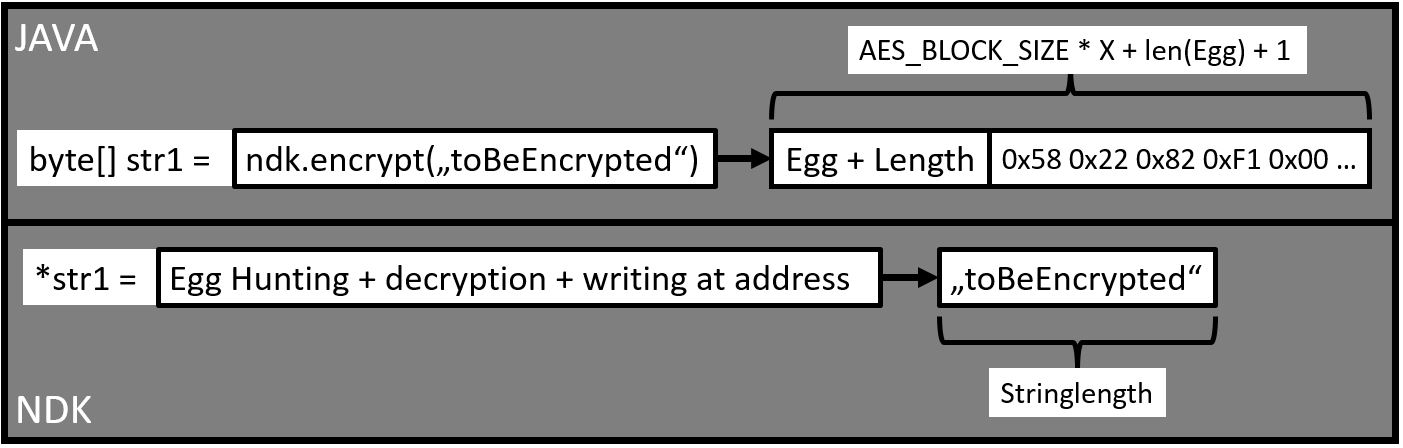
\includegraphics[scale=0.4]{figures/enc_dec_ndk}
  \caption[Dynamic Content Decryption using Eggs]{Dynamic Content Decryption using Eggs}
  \label{fig:enc_dec_ndk}
\end{figure}

Instead, another approach would be to perform the whole encryption/decryption
in native code while programming the logic in Java. The work flow for the developer would be like this: Strings are being defined as byte arrays by initializing them by calling the corresponding NDK method for encrypting
returning the encrypted bytes. App objects of the App can use those bytes
as they were strings by using a ``\code{new String(bytes)}'' call.
After checking the license of the App, those byte arrays can be replaced
with bytes returned by the NDK decryption method. \autoref{ndk_enc_dec}
shows the example App and the corresponding NDK calls to show their signature.
\begin{lstlisting}[language=Java, caption=NDK Encryption/Decryption, label=ndk_enc_dec]
static final MyNDK ndk = new MyNDK();
public class MainActivity extends AppCompatActivity {
    byte[] cbytes = ndk.encrypt("toBeEncrypted","secretkeyxxxxxxx");

    protected void onCreate(Bundle savedInstanceState) {
        super.onCreate(savedInstanceState);
        setContentView(R.layout.activity_main);
        final TextView eggText = (TextView)findViewById(R.id.textView);
        eggText.setText(new String(cbytes));

        //license check
        if (isLicensed()){
            eggText.setText(ndk.decrypt(cbytes,"secretkeyxxxxxxx"));
        }
    }
}
\end{lstlisting}
\autoref{ndk_enc_dec} makes clear that again one call (\code{isLicensed()}) is
responsible for transforming an App to have readable content since the key
is hard-coded in this case and would therefore be again the weak spot. AES
was used for encryption/decryption which is a symmetric method for a proof of concept. To make this technique more secure, one could fetch the decryption
key inside of the \code{isLicensed()} method so that even by avoiding that
license call, the text still would remain encrypted. This can be achieved
by using an asymmetric encryption technique for instance ``ElGamal''.
The encryption key could then be hard-coded since the private counterpart
to decrypt would be missing. Another solution would be to not even encrypt
those strings in source code but with another program/script and only inserting the outcome - the encrypted bytes.
Then also a symmetric technique like AES can be used
after fetching the decryption key when being licensed. In the authors opinion
that would be the most secure solution since the string to be encrypted
would not even appear anywhere in the DEX or in memory as clear text
(sweeping over the memory reveals that the to encrypted string in assignment
\code{ndk.encrypt("toBeEncrypted","secretkeyxxxxxxx");'')} is being present
in memory and could also be present in the DEX).
The downside of course is a bit of comfort for the developer since he would
call an encryption script for every string he does want to use and copying
those bytes into his Java source code.
The NDK C++ AES encryption/decryption methods can be found in \autoref{chapter:ndk_aes_implementation}. OpenSSL libraries are present in Android but are
not intended to be used by the NDK. So it can either be built manually
like explained in \parencite{openssl_building} or using a pre-compiled version
for instance from \parencite{openssl_precompiled}. Android Studio's makefiles
need to be adapted in order to link those libraries.
The AES implementations shown in \autoref{chapter:ndk_aes_implementation} are
using the precompiled version (it's only precompiled for armeabi-v7a as
well as for x86).

Overall, string encryption can be implemented quite secure. The question is
if strings are really a crucial part of an App that needs to be protected.
On the other side, this technique is not limited to strings but can also
be applied to any other App content. Doing crucial parts in native code
like fetching decryption keys or doing the actual encryption/decryption
should increase the reverse code engineering resistance. Due to time
constraints this evaluation can not be performed. Of course the NDK is not
mandatory for such a encryption/decryption technique but can add another
layer of complexity from an attacker's point of view.
